\documentclass[a4paper, 10pt]{article}
\usepackage[utf8x]{inputenc}
\usepackage{graphicx}
\usepackage{mathenv}
\usepackage{amsmath}
\usepackage{geometry}
\geometry{hmargin = 2.5cm, vmargin = 1.5cm}

% OPENING
\title{SY19 - TP03\\Réseaux de Neurones : Optimisation de l'Architecture}
\author{Alice Ngwembou - Antoine Hars}

\begin{document}

\maketitle

\section*{Introduction}
Le but de ce TP est la mise en oeuvre d'un algorithme basé sur les réseaux de neurones pour la classification.

\section*{Exercice 1}

\section*{Exercice 2}

\subsection*{Travail Préliminaire}

\subsubsection*{Question 1 :}

\textbf{1. Quelles sont les 4 lois utilisées pour générer les observations de l’ensemble d’apprentissage appartenant à 4 places ?}\\
Nous avons 4 lois Normales $\mathcal{N}(\mu_{1}, \Sigma_{1})$, $\mathcal{N}(\mu_{2}, \Sigma_{2})$, $\mathcal{N}(\mu_{3}, \Sigma_{3})$ et $\mathcal{N}(\mu_{4}, \Sigma_{4})$ avec :\\ \\
\hspace*{0.5cm}
\begin{tabular}{cccc}
$\mu_{1}$ = (4, 6) &
$\Sigma_{1} = \begin{pmatrix} 1 & 0 \\ 0 & 2 \end{pmatrix}$ &
$\mu_{2}$ = (6, 1) &
$\Sigma_{2}$ = $\begin{pmatrix} 2 & 0 \\ 0 & 1 \end{pmatrix}$\\ \\
$\mu_{3}$ = (-4, 4) &
$\Sigma_{3}$ = $\begin{pmatrix} 1.5 & 0 \\ 0 & 2 \end{pmatrix}$ &
$\mu_{4}$ = (0, 0) &
$\Sigma_{4}$ = $\begin{pmatrix} 1 & 0 \\ 0 & 1 \end{pmatrix}$\\
\end{tabular}\\ \\ \\
\textbf{2. Donner la règle de Bayes qui permet de répondre à un problème de classification à $c$ classes.}\\
La formule de Bayes donne la probabilité, dîte probabilité $a$ $posteriori$, pour qu'un individu décrit pas le descripteur $x$ appartienne à la classe $k$ :
$P(c_{k}|x) = \frac{f_{k}(x)}{\sum{f_{i}(x)}} = \frac{Pr_{k} * f_{k}(x)}{\sum{}Pr_{i} * f_{i}(x)}$, où $c$ est le nombre de classes et $Pr_{k}$ est la probabilité $a$ $priori$ que l'individu appartienne à la classe $k$.\\ \\
\textbf{3. Développer la règle de Bayes pour arriver à la solution donnée dans le code ci-dessus.}\\
Pour appliquer la formule de Bayes, on calcule les densités de probabilité de chacune des lois qu'on multiplie à leur probabilité $\pi$, ce qui nous permet de les comparer entre elles pour chaque point.\\
Cela se traduit dans le code R par la définition d'une grille sur le graphique qui nous permet de comparer la probabilité d'appartenance à l'une des lois en chacun des points de cette grille. Ce traitement nous permet de récupérer et d'afficher (au moyen de la fonction $contour$) le contour de chacune des densités supérieure à 0 des 4 classes.

\subsection*{Réseaux de neurones sur des données simulées}

\subsubsection*{Question 2 :}

\textbf{1. Dessiner le frontières de décision obtenues avec un réseau de neurones sur les données (pour decay = 0 et size = 5.)}\\
L'exécution du code donnée nous permet d'observer le graphique suivant :\\
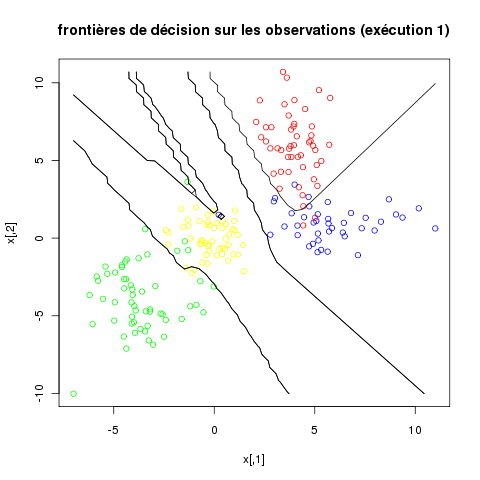
\includegraphics[height = 7cm, width = 7cm]{plots/frontiere_bayes_q2_1.png}\\
Nous pouvons observer sur ce graphiques les différentes observations de l'ensemble d'apprentissage avec une couleur précise et les frontières de décision obtenues.\\
On peut dire que tous les points de chaque loi normale ne se situent pas exactement du bon coté des frontières de décision.\\
Donc il y a une certaine probabilité d'erreur qu'un individu appartienne à une classe.\\ \\
\textbf{2. Visualiser l'estimation des poids.}\\
L'estimation des poids pour decay = 0 et size = 5 nous donne le graphique suivant :\\
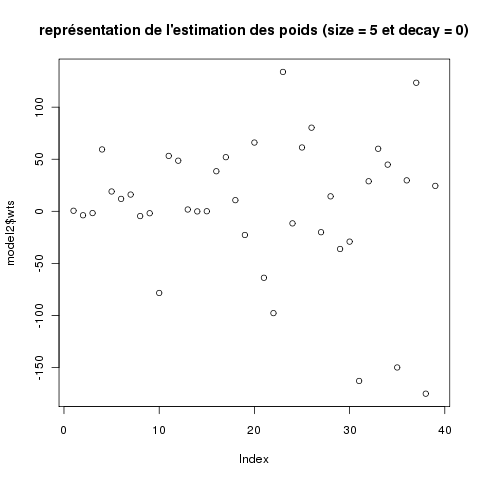
\includegraphics[height = 7cm, width = 7cm]{plots/poids_q2_2_1.png}
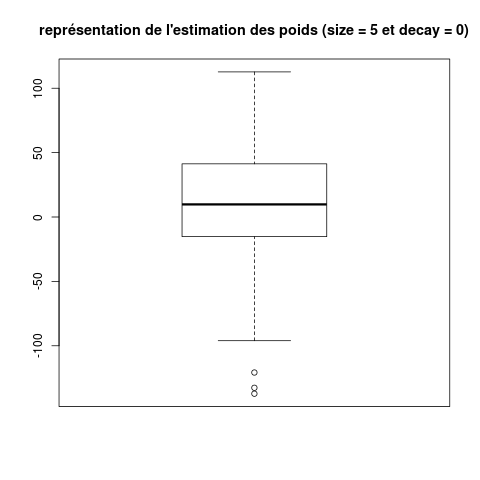
\includegraphics[height = 7cm, width = 7cm]{plots/poids_q2_2_2.png}\\
On peut voir que la majorité des poids sont compris entre -40 et 40.\\ \\
\textbf{3. Obtient-on les mêmes résultats à chaque fois pour l'estimation des poids et des frontières de décision lorsqu'on lance plusieurs fois la procédure $nnet$ ?}\\
En relançant la procédure $nnet$, nous n'obtenons pas les mêmes frontières de décision.\\
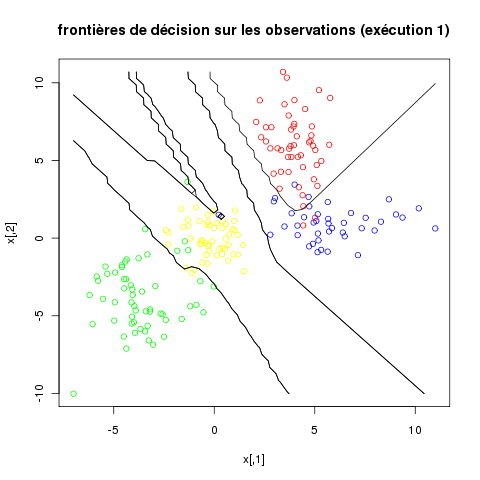
\includegraphics[height = 7cm, width = 7cm]{plots/frontiere_bayes_q2_1.png}
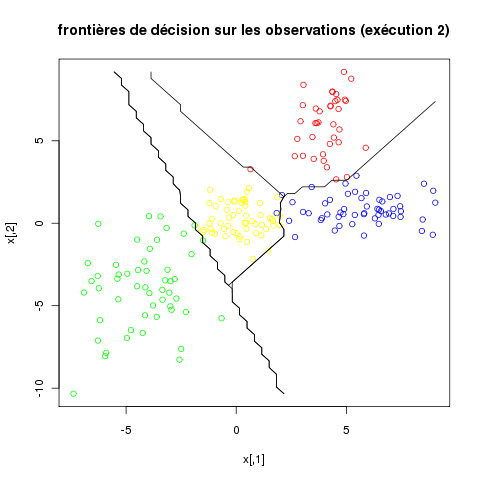
\includegraphics[height = 7cm, width = 7cm]{plots/frontiere_bayes_q2_2.png}\\
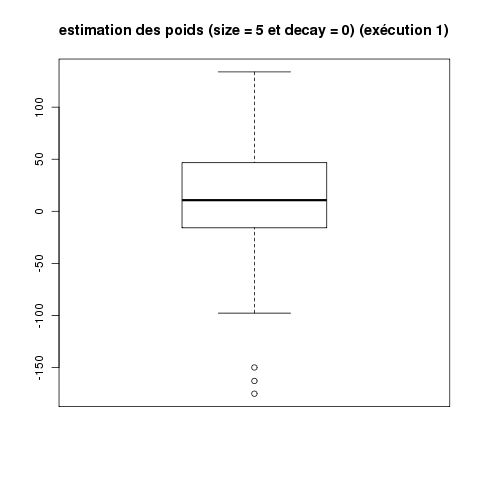
\includegraphics[height = 7cm, width = 7cm]{plots/poids_q2_2_3.png}
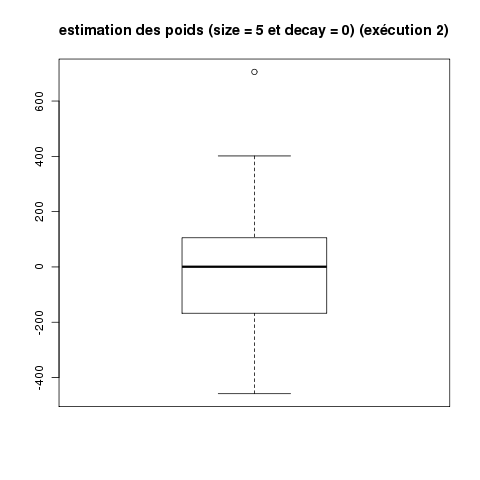
\includegraphics[height = 7cm, width = 7cm]{plots/poids_q2_3_2.png}\\
Nous pouvons observer que les probabilités d'erreur ne semblent pas les mêmes entre les 2 exécutions mais que les frontières séparent assez bien les différentes classes.\\
Du coté de l'estimation des poids, nous obtenons des valeurs plutôt semblables entre -50 et 50 mais que pour les valeurs extrèmes, il n'y a pas du tout le même ordre de grandeur.\\ \\
\textbf{4. Comment expliquer ce phénomène ?}\\
il semble que ce phénomène vient du fait que le générateur de nombre aléatoire de R n'est pas réinitialisé entre les 2 exécutions de $nnet$, car nous utilisons la méthode de rétro-propagation dans cet algorithme qui contient une initialisation au préalable des poids dans le réseau de neurones avec des valeurs aléatoires. Cet valeurs aléatoires sont donc assujetties à la bonne initialisation du générateur de nombres aléatoires de R.

\subsubsection*{Question 3 :}

On désire voir l'influence du nombre de neurones dans la couche cachée. Pour cela, pour decay = 0, faire varier size de 1 à 10 (nombre de neurones dans la couche cachée).\\ \\
\textbf{1. Commenter le nombre de "poids" à estimer.}\\
La variation de $size$ nous donne les graphiques suivants par rapport à l'estimation des poids optimaux :\\
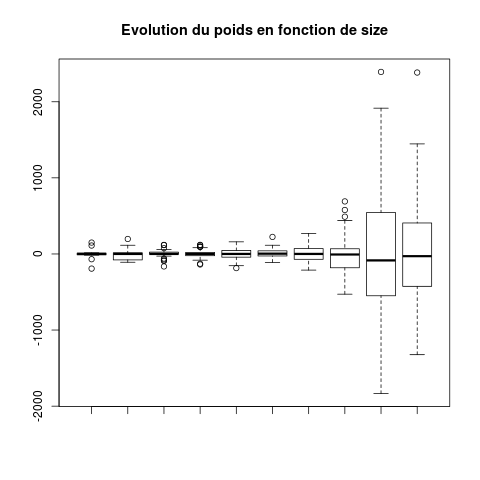
\includegraphics[height = 7cm, width = 7cm]{plots/poids_q3_1.png}
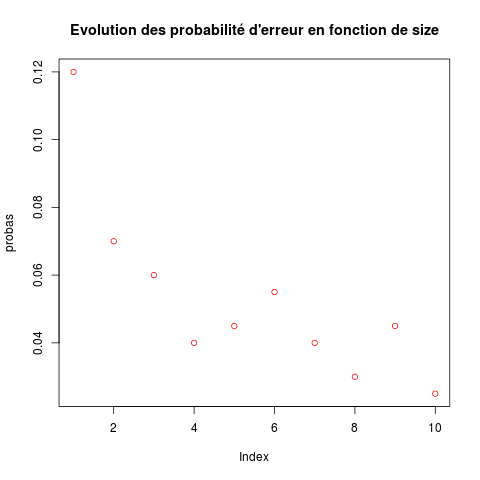
\includegraphics[height = 7cm, width = 7cm]{plots/probas_erreur_q3_1.png}\\
Nous pouvons observer que pour les plus grandes valeurs de $size$, la probabilité d'erreur sur les poids optimaux est très faibles.
Si le nombre de neurones cachés est faible, il y a une plus grande chance qu'un point soit mal classé.\\
On observe, sur l'estimation des erreurs en fonction de $size$, que la probabilité d'erreur diminue entre 1 et 4, puis remonte pour redescendre entre 6 et 8, remonter pour $size$ = 9 et enfin être très basse pour une valeur de $size$ égale à 10.\\ \\
\textbf{2. Afficher les frontières de décision (4 seulement). Que constater sur la forme des frontières et sur le nombre de points mal-classés quand size augmente ?}\\
Nous choisissons donc d'afficher les frontières de décision pour $size$ égal à 1, 4, 6 et 10 d'après l'évolution des probabilités d'erreur vue précédemment.\\
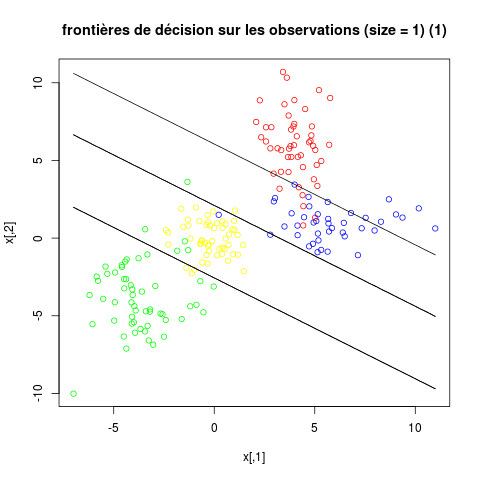
\includegraphics[height = 7cm, width = 7cm]{plots/frontiere_bayes_q3_2_1.png}
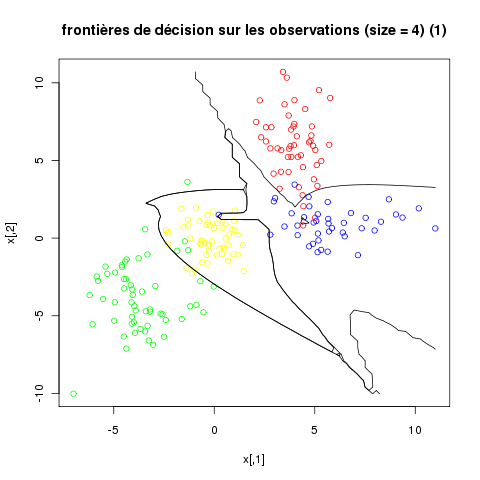
\includegraphics[height = 7cm, width = 7cm]{plots/frontiere_bayes_q3_2_4.png}\\
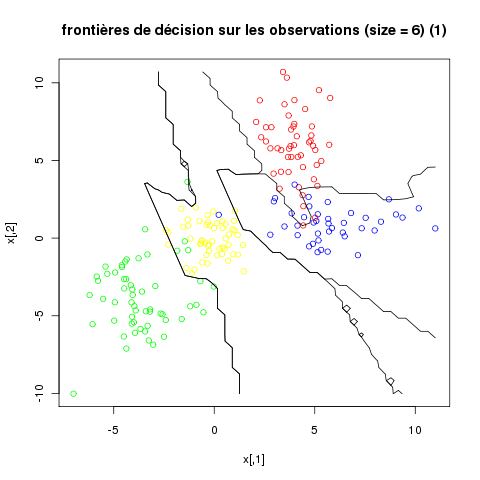
\includegraphics[height = 7cm, width = 7cm]{plots/frontiere_bayes_q3_2_6.png}
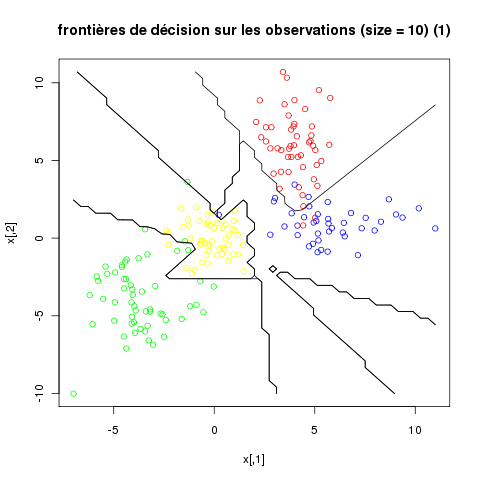
\includegraphics[height = 7cm, width = 7cm]{plots/frontiere_bayes_q3_2_10.png}\\
Pour le premier graphique, où la probabilité d'erreur est la plus élevée, les frontières de décision sont des droites donc le nombre de points mal-classé se retrouve à être assez conséquent par rapport aux autres graphiques dont les frontières de décision sont des courbes.\\
On remarque plus $size$ augmente, plus les courbes sont complexes. Par exemple, entre le troisième et le quatrième graphique, l'inclusion ou non du point bleu au dessus des points jaunes sur les graphiques, montre la complexité du modèle et nous confirme les valeurs des probabilités d'erreur du mauvais classement d'un point du modèle. $size$ = 4 est plus précis que $size$ = 6 mais moins précis que $size$ = 10. 
\textbf{3. Relancer la procédure sur un nouveau jeu de données en faisant varier size de 1 à 10.}\\
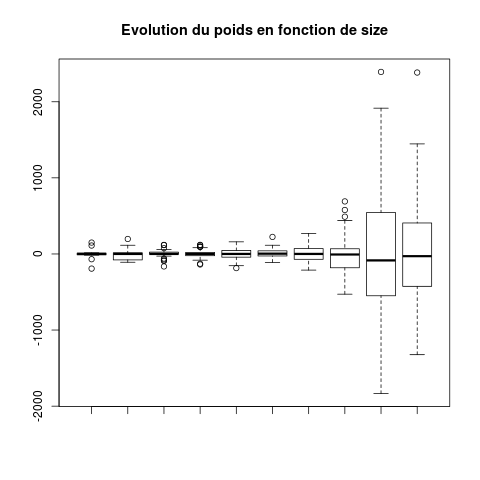
\includegraphics[height = 7cm, width = 7cm]{plots/poids_q3_3.png}
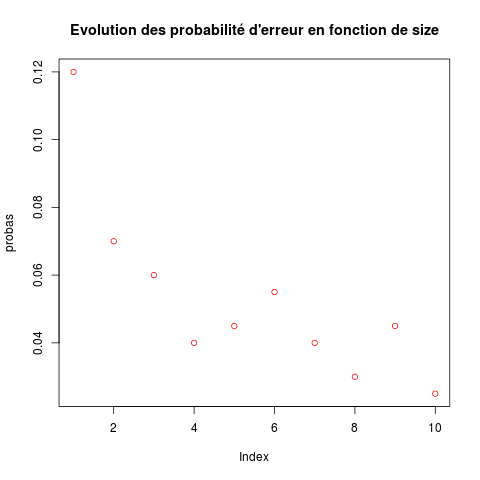
\includegraphics[height = 7cm, width = 7cm]{plots/probas_erreur_q3_3.png}\\
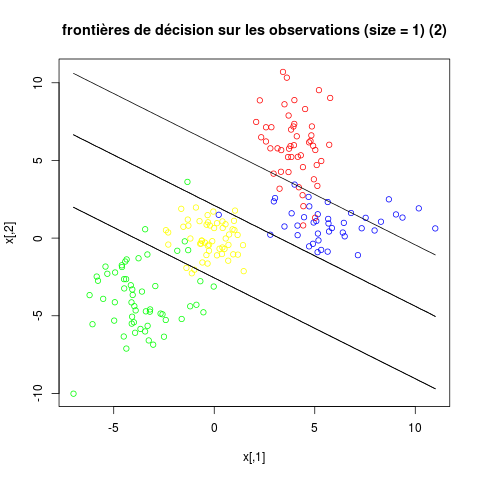
\includegraphics[height = 7cm, width = 7cm]{plots/frontiere_bayes_q3_3_1.png}
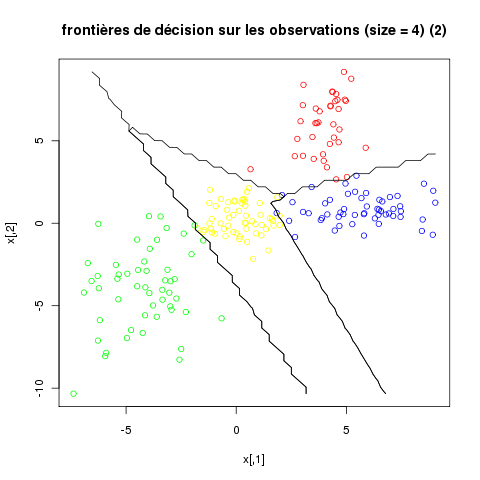
\includegraphics[height = 7cm, width = 7cm]{plots/frontiere_bayes_q3_3_4.png}\\
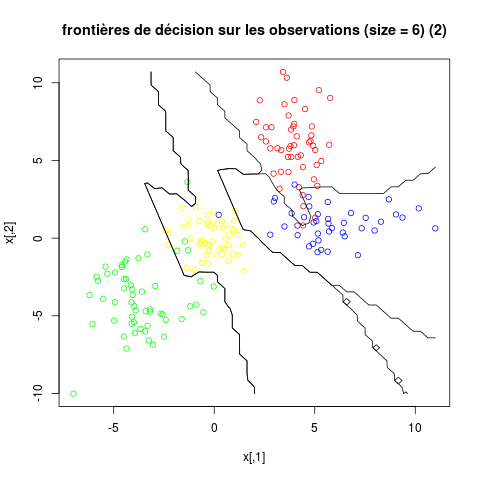
\includegraphics[height = 7cm, width = 7cm]{plots/frontiere_bayes_q3_3_6.png}
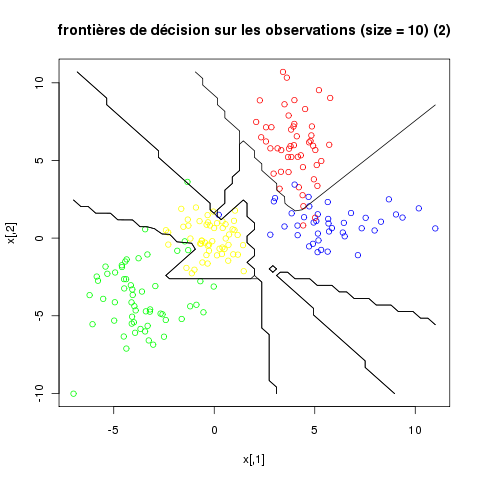
\includegraphics[height = 7cm, width = 7cm]{plots/frontiere_bayes_q3_3_10.png}\\
Nous pouvons observer que les frontières de décision et les estimations des poids optimaux ne changent pas avec un nouveau jeu de données du fait que nous veillons à ré-initialiser le générateur de nombre aléatoire du logiciel R avant tout exécution de l'algorithme.\\ \\
\textbf{4. Que dire de la variabilité du modèle en fonction de size ?}\\
Plus la taille du réseau de neurone augmente, plus les frontières de décision seront complexes et précises, la probailité qu'un point soit mal-classé est plus faible lorsque $size$ augmente.\\
Cependant, nous avons observé que lorsque le nombre de neurones cachés se rapproche de la valeur du nombre lois utilisées pour fournir l'ensemble d'observation, la probabilité d'erreur de l'appartenance d'un point à une classe est plus faible que pour les valeurs de $size$ adjacentes.

\subsubsection*{Question 4 :}

On désire voir l'influence du paramètre de régularisation $decay$ qui influe sur la précision du modèle.\\ \\
\textbf{1. Pour size = 5, comparer l'estimation des poids et des frontières pour decay = 0.001, 0.01, 0.1, 1, 10, 100.}\\
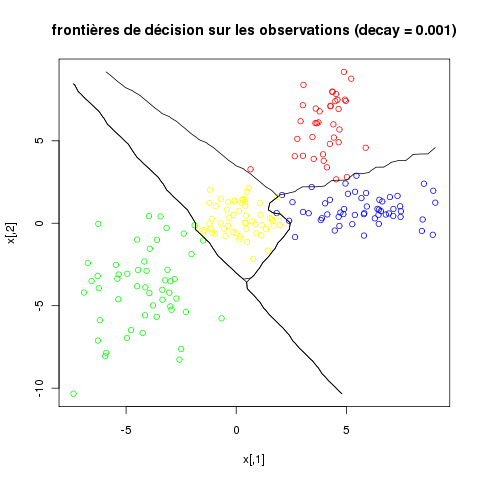
\includegraphics[height = 7cm, width = 7cm]{plots/frontiere_bayes_q4_1.png}
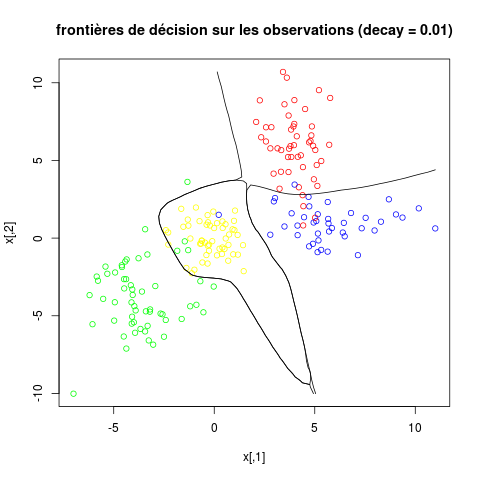
\includegraphics[height = 7cm, width = 7cm]{plots/frontiere_bayes_q4_2.png}\\
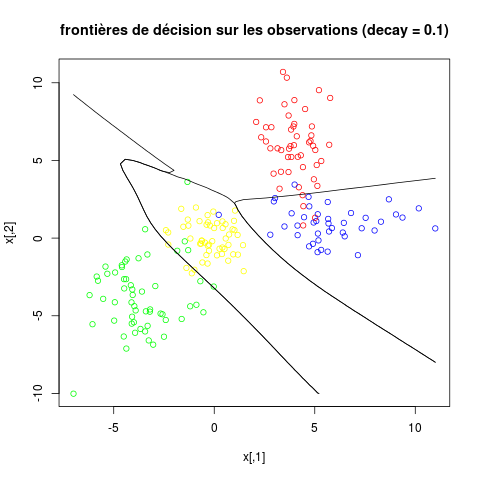
\includegraphics[height = 7cm, width = 7cm]{plots/frontiere_bayes_q4_3.png}
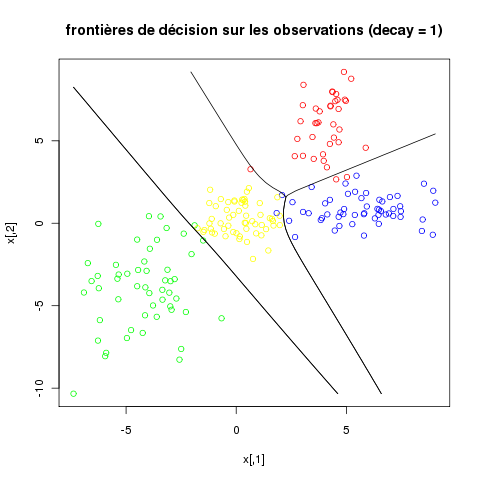
\includegraphics[height = 7cm, width = 7cm]{plots/frontiere_bayes_q4_4.png}\\
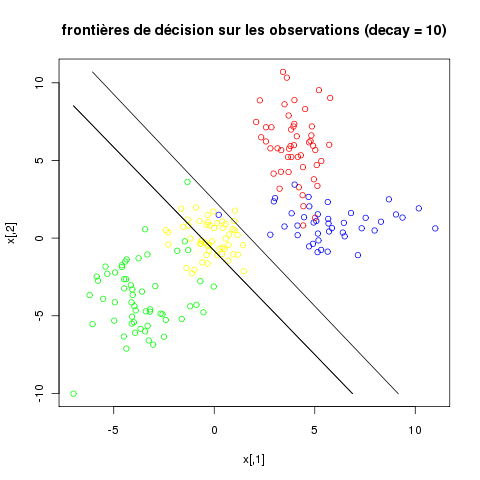
\includegraphics[height = 7cm, width = 7cm]{plots/frontiere_bayes_q4_5.png}
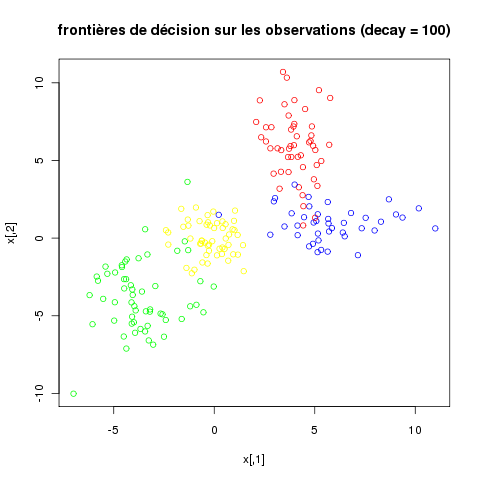
\includegraphics[height = 7cm, width = 7cm]{plots/frontiere_bayes_q4_6.png}\\
Pour la représentation des frontières de décision suivant les différentes valeurs du paramètre de régularisation, nous pouvons observer que plus la valeur de $decay$ est grande, moins les frontières de décision sont précises. Pour une valeur de 100, nous n'avons même plus de frontières de décision, tandis que pour une valeur de 10, les frontières sont très peu précises (nous avons juste 2 droites séparant approximativement les classes). Pour les valeurs très petites de $decay$, les frontières de décision font plus attention au découpage des classes par rapport à l'intersection des classes.\\ \\
L'estimation des poids associés aux différentes valeurs de $decay$ nous donne les graphiques suivants :\\
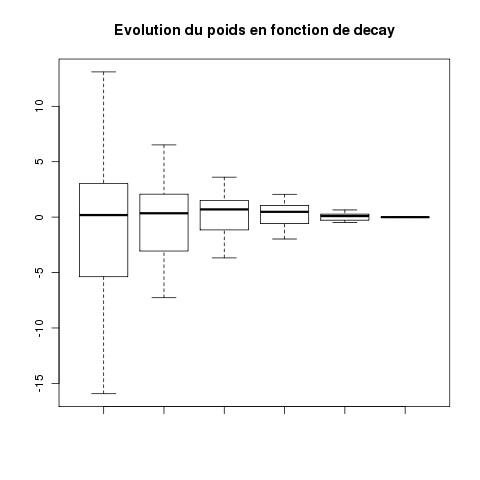
\includegraphics[height = 7cm, width = 7cm]{plots/poids_q4_2.png}
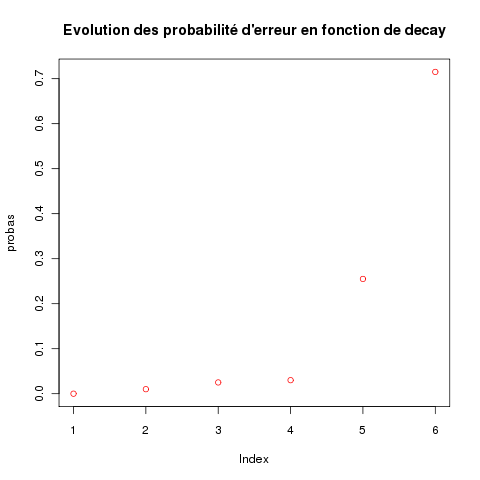
\includegraphics[height = 7cm, width = 7cm]{plots/probas_erreur_q4_3.png}\\
On remarque que plus la valeur du paramètre de régulation augmente, plus les poids se rapprochent de 0 et que la probabilité d'erreur augmente si $decay$ est grand.\\ \\
\textbf{2. Que dire de la valeur des poids optimaux quand $decay$ augmente ?}\\
On peut voir sur le graphique des probabilités d'erreur en fonction de $decay$ que pour des valeurs comprises entre 0.001 et 1, les probabilité d'erreur n'excède pas 10\%, ce qui donne donc des valeurs de poids optimaux plutôt intéressantes alors que pour des valeurs supérieures à 1, la probabilité d'erreur augmente beaucoup pour être à environ 32\% pour $decay$ = 10 et 72\% pour $decay$ = 100 ce qui ne nous donne pas des valeurs de poids optimaux vraiment probant.\\
Nous pouvons faire le lien de ces observations avec le $boxplot$ de l'évolution du poids en fonction de $decay$ où nous avons des boîtes à moustache dont les quartiles sont tous proches de zéro pour les 2 dernières valeurs du paramètre de régularisation, donc les 2 valeurs les moins probantes pour avoir un modèle convenable. Pour une faible valeur de $decay$, les valeurs de poids varient beaucoup, avec une forte amplitude.\\ \\
\textbf{3. Comment expliquer ce phénomène et comment cela se traduit-il sur la forme des frontières ?}\\
Ce phénomène provient de l'ajout d'un terme de pénalisation $P$ au critère d'erreur $R$ sur la régulation du modèle : $C = R + \lambda P$, $\lambda$ étant un $hyperparametre$.
Plus la valeur de $decay$ est petite, plus le modèle proposé est complexe, alors que plus elle est grande, le modèle sera plus généraliste et simple. Au niveau des frontières de décision, cela se traduit pas des frontières très précises pour un $decay$ proche de 0 et des frontières moins précises, plus droites pour un grand $decay$. Pour un $decay$ trop élevé, il n'y a plus de frontières.

\subsection*{Classification des données Crabes}

\subsubsection*{Question 5 :}

\subsubsection*{Question 6 :}

\section*{Conclusion}

\end{document}
